\chapter{Introduction}
\section{Motivation}
    
  Sight is one of the most fundamental senses we - humans- posses. \todo{stats about vision, and the interesting paper I found on visual ensemvles and summary statistic} Our brains are evolved to process information quickly to allow us to reason with this information and react external stimuli. We also rely heavily on this skill to navigate the world; make sense of the unknown by observing it. Robots are no different. As the robotics industry evolved over the many decades, Computer Vision \todo{ref somethinhg} Based solutions became a staple in allowing machines to \emph{see}.

  Reinforcement \todo{ref} and Imitation Learning \todo{ref} are two prominent methods in tuning such visual robots. Where a robot will be fitted with an assortment of cameras and sensors to perceive its environment. These cameras can be mounted in many configurations: Mounted on their wrists \cite{chi2024UMIinthewild,openXEmbodimentRoboticLearning2024}, over the shoulder \cite{wang2024observeactasynchronousactive}, or in some cases placed around the environment \cite{exploringActiveVision2024chuang} that the robot is interacting to allow entire scenes to be observed. These configurations are not mutually exclusive and multiple can be used to maximise information gain. A major problem this introduces is cost and mobility:
  \begin{itemize}
    \item Third-person cameras are challenging to incorporate into non-static tasks. And on-body solutions, like wrist-mounting, provide limited visual understanding with occlusions and increased environmental entropy becoming a challenge. 
    \item Multi-view setups are usually big and clunky \todo{ref here}, losing on dexterity and more importantly stop being general-use robots
  \end{itemize} 

  To take inspiration from humans: we use our eyes which can be operated independently from our other extremities. This optimising aspect of human visual feedback \cite{findlay2003active,maiello2021humans,goodman2018using} is one of the cornerstones of human learning and environment manipulation. Take, for example, a USB stick and its port. It is unlikely (impossible even) to ensure success in the first insertion attempt. However, shifting our view to make sure the port, the USB stick, and our hand are \emph{in-frame}, meaning we can see them clearly. The success rate of the next attempt sky-rockets.
  
  Therefore, a possible solution to robot observation uncertainty is to actively explore the environment and understand the environment before acting. In this project I will explore what it means for a robot to view and understand what it is seeing. And explore geometric reasoning and uncertainty ensemble methods to overcome problems arising from static observations.


\section{Contributions}
  This is an experimentation-driven project. With end goal being of understanding 3D tasks and robots' reasoning of them to create competent active vision policies. The work is laid out as follows:

  \begin{itemize}
    \item Explore CoppeliaSim and propose some reaching and grasping tasks for training my policies on (Sections \ref{sec:3d-reaching-tasks}, \ref{sec:grasping-tasks}, \ref{sec:reach-obs})
    \item Propose and explore ideas of feature fusion to increase the learning potential and the competency of robot policies (Sections \ref{sec:depth-interfacing}, \ref{sec:multi-modal-policies}, \ref{sec:proposed-fusion})
    \item Design and reason about the foundations of two active vision policies and their implementations (Chapter \ref{ch:appl})
    \item Finally, evaluate and compare the competencies and potential drawbacks of the various policies and feature fusion methods (Chapter \ref{ch:eval})
  \end{itemize}


  On this visual information we can train control policies for robots using Neural Networks \cite{spyros1995nnStateOfTheArt, Schmidhuber2015nn} -of differing architectures- that are fit for the task we need our robot to do. However, these methods of mounting cameras comes with various disadvantages:
  
  \textbf{Static Cameras} Environment observing static cameras, such as over-the-shoulder (third-person) mounted cameras mean that the robot is confined to its environment and occlusions are still possible depending on the angles and the number of such cameras placed.
    
  \textbf{Camera-in-hand} This method can suffer from similar issues. As the gripper is oriented to execute a task, the viewpoints the camera sees will change. This dependency means that select tasks that are inherently occluding, once the gripper is engaged; for example, screwing in a lightbulb, inserting a key \ldots This means that optimal learning cannot be achieved for such a robot. As we get partial observability of the Region of Interest (ROI) at best and complete occlusion of the ROI at worst. See example in Figure \ref{fig:ex-occlusion} and Figure \ref{grid-occlusion}.

  \begin{figure}[h]
    \centering
    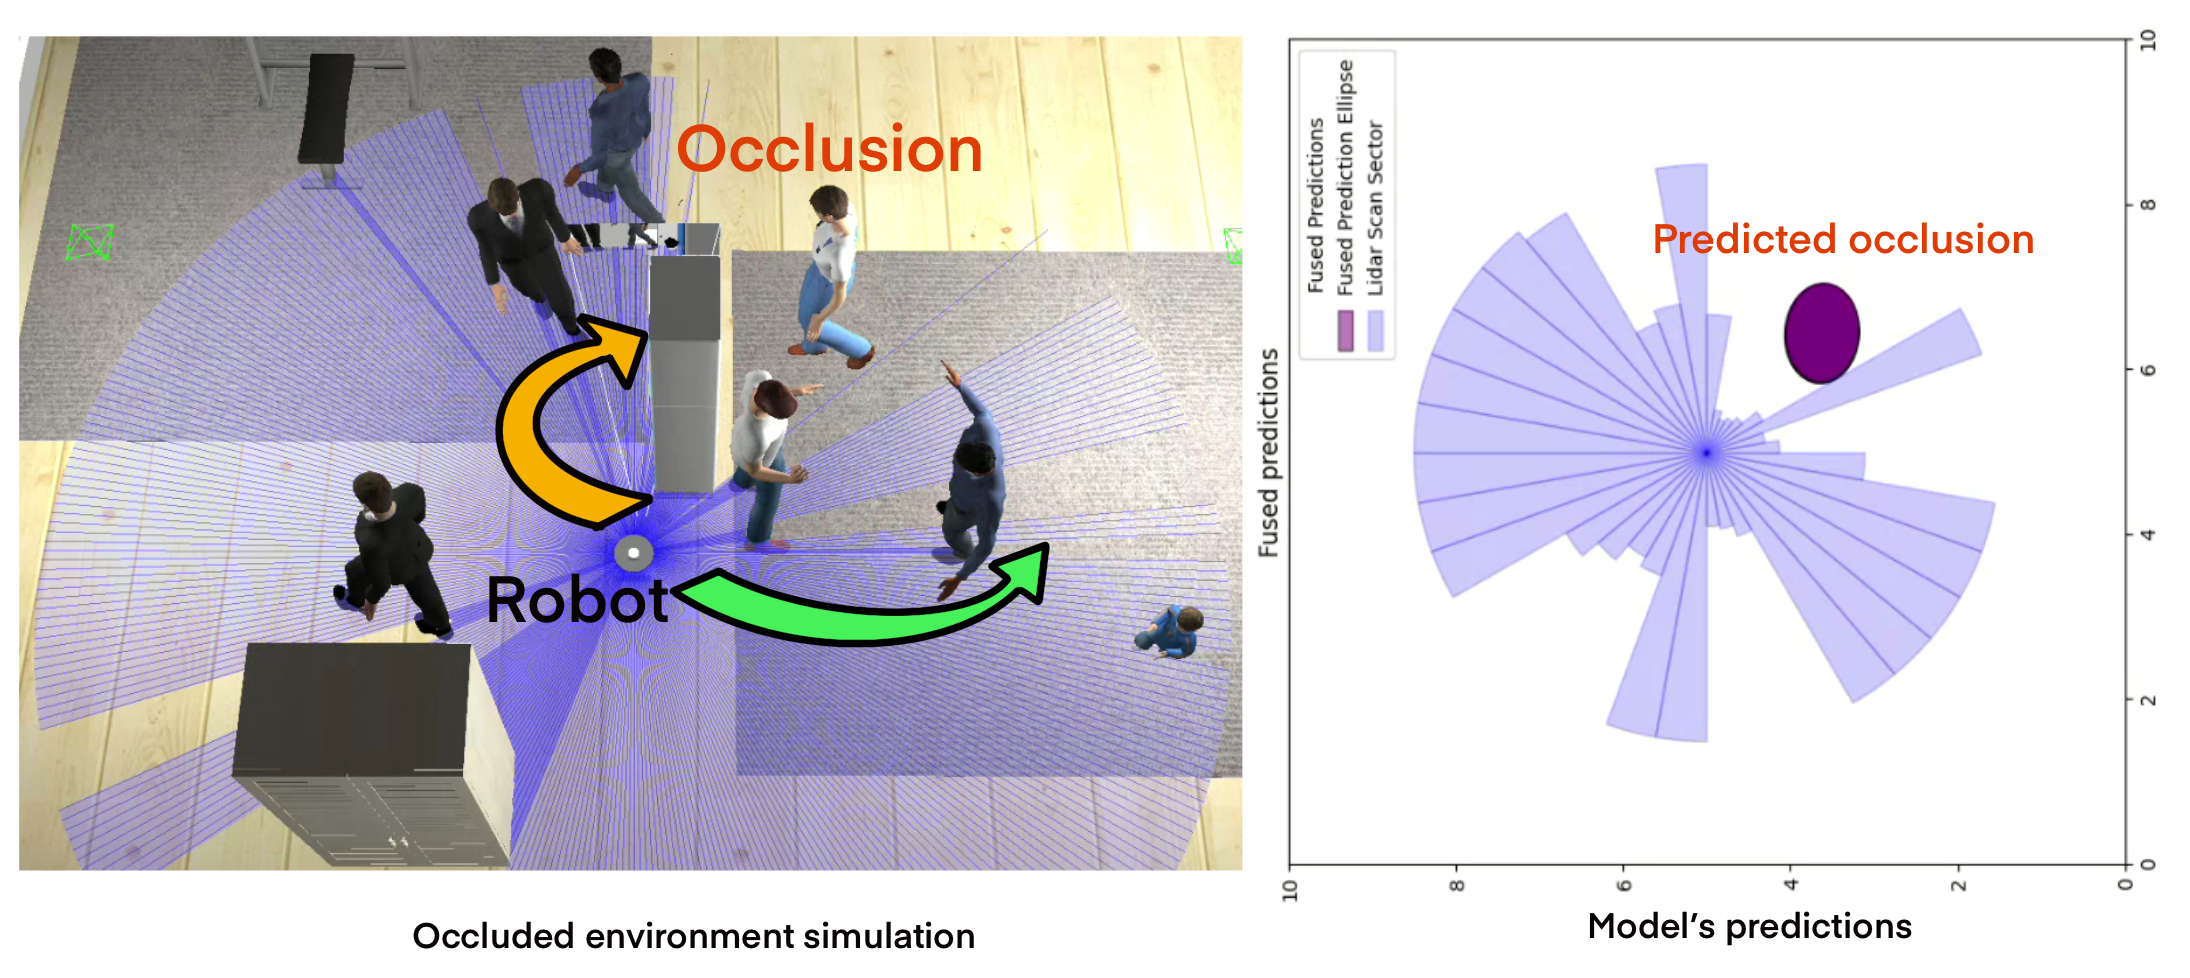
\includegraphics[width=0.7\textwidth]{assets/intro/intro-occlusion.png}
    \caption{Example of a robot mapping occluded areas \cite{ranaraja2024occlusionawareobstacleprediction}}\label{fig:ex-occlusion}
  \end{figure}
    
  In contrast to the above, us humans use our eyes which can be operated independently from our arms.  So, a possible remedy of the above issues is having a free moving, controllable camera alongside a interactive live (i.e. a gripper). This human-like setup -with the grippers as the arms and the camera arm as the neck, head and eyes- now allows our robot to find optimal camera poses for the tasks at hand and gain the most information about a scene.
  
  This now means that the \emph{visuomotor} tasks, where robot stimuli are controlled according to observations, shift to that of an \emph{Active Vision} one. This is a highly active area of research in robotics and mostly tackled through synchronous video with teleoperation \cite{exploringActiveVision2024chuang} with Behavioural Cloning, where a human \emph{pilot}will control the robot through some sort of interface, like a virtual reality (VR) headset. So the robot can learn to move its viewpoints according to this pilot's demonstrations. Another avenue of exploration is asynchronous vision, where the vision and movement information is learnt separately but coupled during execution of the robot \cite{natarajan2021graspsynthesisnovelobjects,wang2024observeactasynchronousactive}.


  \begin{figure}[h]
    \centering
    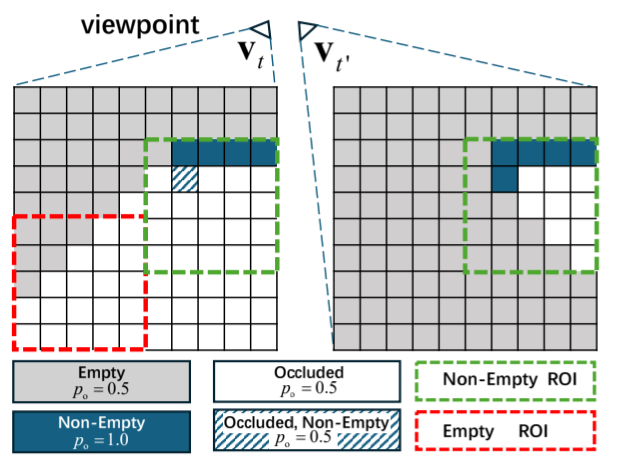
\includegraphics[width=0.8\textwidth]{assets/intro/grid-occluded.png}
    \caption{Example of multiple viewpoints gathering different information \cite{wang2024observeactasynchronousactive}}\label{fig:grid-occlusion}
  \end{figure}
  \todo[color=green]{make a better image for final}

  So our goal in this project is to explore how a robot can learn end-to-end control policies while also learning an active vision policy to optimise the movement of the camera during execution of tasks. And how this compares to existing methods of learning policies, with or without active vision approaches, and possibly its prevalence in real world scenarios. 

\section{Objectives}\label{sec:intro-objectives}
    So, the plan of this project then is to investigate whether a robot can be made to learn an active vision policy around the task it is currently being instructed (Imitation) or is currently exploring with some reward (Reinforcement).
    \todo[color=green]{Could change depending on where we get to exploring, I think the intereting ones are 2 and 3, 1 seems to be done a few times}

    We are therefore proposing three ways to investigate this:
    \begin{enumerate}
      \item Robot learns a policy as normal. Then during policy execution, the robot uses 3D-reasoning and forward planning, in order to predict its optimal pose so that the object(s) of interest are clearly visible and not occluded by other objects.
      \item The robot randomly moves its camera around during the policy learning in order to generate a range of different camera viewpoints (for the same robot states). When the policy is deployed, the uncertainty of the policy can be used to guide the camera towards regions with low uncertainty.
      \item In simulation, reinforcement learning is used to train a policy that directly controls the camera, for any given task and object, using randomly generated "pseudo-tasks". Then after training a robot on a task using human demonstrations in the real world. Two policies will be deployed: the main policy controlling the robot's hand, and the policy controlling the robot's camera.
\end{enumerate}
% \todo[color=green]{testing should be done on real life and simulated scenarios alike}
% Following on from the results of a predetermined test suite we can then determine what is the most promising model out of the three and develop them further.
% \section{Scope}
% \todo{Not sure if this is needed for Interim report, will come back}
% !!Not sure if this is needed, following are some things I thought could be included here for the final project report.

% \begin{itemize}
% 	\item Types of tasks the project will cover
% 	\item assumptions, camera, robot, arm types etc
% 	\item predetermined test suite maybe?
% 	\item distinction between control policies for the hand arm (policy for task) and the camera (optimal view)
% \end{itemize}

% \todo[color=red]{info edward wanted check teams}